\section{Exchange Transactions}
\label{section:exchange_transactions}

% \subsection{Markets}

% One effort to explain the sustained failure or markets to equilibriate at the aggregate level is to
% try to explain failure of equilibriation as a result of the way individual economic behaviour
% aggregates to failure or otherwise of markets for single products to equilibriate, and further to
% explain failure of markets to equilibriate at the aggregate level.
% 
% A fundamental method of science and engineering is to assume as a first step, is to use the mean
% value to aggregate a collection of micro-level behaviours. Often this turns out not to be correct,
% but invariably, in virtually every system we seek to explain, there are some parts of the system we
% explain away by averaging out noisy behaviour. 
% 
% If we use the same technique for understanding economic behaviour, we would, as a first step assume
% that we can average markets for single goods or services, result in an aggregate supply or demand
% close to zero.
% 
% If we use the same technique for understanding economic behaviour, we would, as a first step assume
% that we can aggregate our model of supply and demand for single goods or services, and arrive at a
% aggregate where aggregate supply or demand is close to zero.
% 
% Since this conclusion is contrary to facts, economists have directed their efforts at modifying the
% supply and demand model in many ways in an effort to explain this contradiction between fact and
% theory.
% 
% What is clear, however, is that the explanation has to be sufficiently fundamental to explain the
% remarkably consistent fact of excess aggregate supply and the rarity of aggregate market
% equilibrium. As put forward by Lucas, economists have yet to find a convincing understanding of
% this fact, let alone to find a solution to the problem of equilibrium failure or the problem of
% a sustained positive unemployment rate. 
% 
% Since our explanation of these facts is outside is not a part of the supply and demand model, we
% assume our simplest model of market behaviour, and that markets at the aggregate level do in fact
% equilibriate, relying on the law of large averages.

\subsection{An Exchange Transaction Only Model}

We will start with a model simplified from Figure \ref{fig:economic_feedback_schema1}. that includes only
exchange transactions.

\begin{figure}[H]
\centering
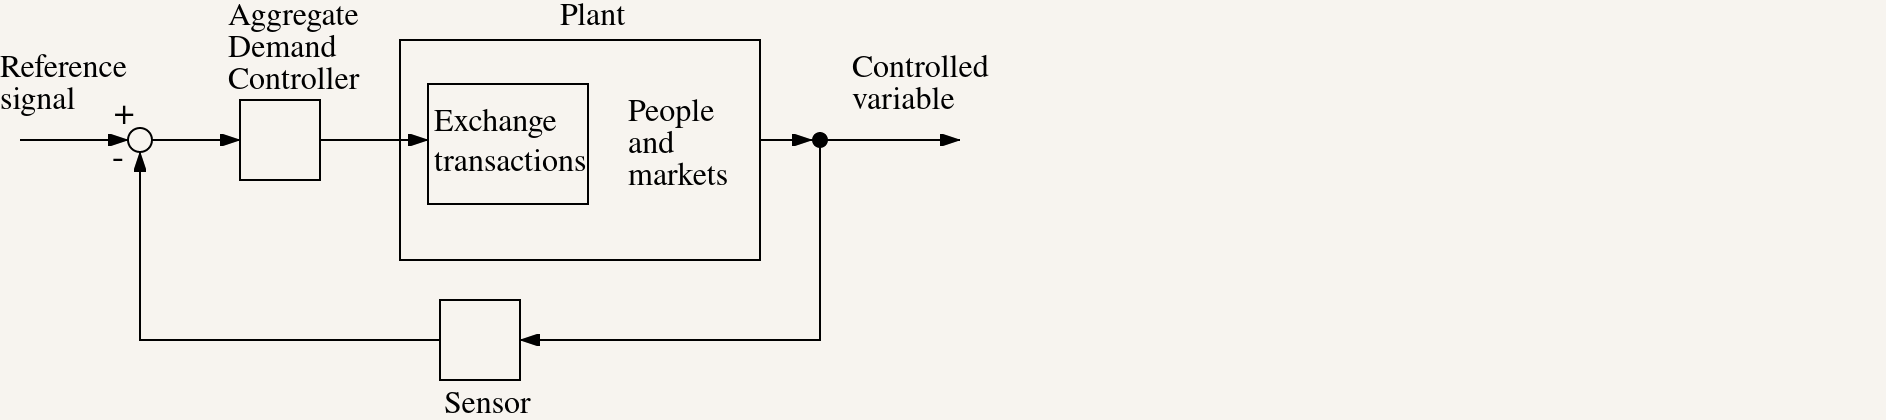
\includegraphics[scale=0.60]{03_exchange_transactions/png/exchange_only_feedback_schema}
\caption{Exchange Only Feedback Schema}
\label{fig:exchange_only_feedback_schema1}
\end{figure}

\subsection{Price and Quantity}

An exchange transactions can be characterized by a payment. We will use the unit ``dollar''
for payments. In exchange for a payments is a quantity of goods or services of a certain goods
category. We denote the quantity with a unit specific to the goods category. The price of the
transaction is the ratio of payment to quantity and the unit is dollars per unit of the goods
category. These variables relate directly to properties of transactions which indicate the state
change in a set of accounts. They are precise and measurable quantities, so we treat them
differently to measures of economic measures which try to handle some notion of human good. We
denote $f_i$ are the sum of payments for a given goods category $i$ over a period of time The unit
for any $i$ is ``dollars''. We denote the quantity of that goods category transacted in
exchange for these payments $q_i$. The unit can be different for each $i$. The average price of each
goods category is 

\[
    p_i = \frac {f_i} {q_i}
\]

We can sum $f_i$ for all transactions in a given period.

\[
    F = \sum_i f_i
\]

As will be shown later, the aggregate value we are interested in is an accurate measure of the price
level such that a person own $x$ dollars now has the same purchasing power at any time in the
future. We need to specify this more precisely.

The quantity and proportion of different goods transacted using a currency changes over time. We use
the notion of purchasing power to construct a measure to handle this.

We can image an ``abstract person'' who we feed a dollar now, and makes random selections of goods
and services to purchase per dollar. This random selection of purchases on average accounts for a
given proportion of the total amount of purchases made during that time period. 

We define the price index that changes over time $P_i$ such that

\[
    \frac {c_j} {P_j} = \frac {c_k} {P_k}
\]

for every time period $j$ or $k$, this equality holds, where $c$ is the average proportion of the
whole amount of transactions that our ``abstract person'' makes. The important point of this
discussion is to present the case that 

\[
    P = p_i \left( \frac {f_i} F \right) + \cdots + p_n \left( \frac {f_n} F \right) = \sum_i p_i
    \left( \frac {f_i} F \right)
\]

where the central measure of price we are looking for is where each purchase is weighted by the
proportion of total payments  for that purchase, as this is the value that would make equation TODO
hold. Now we want to see how $P$ and $F$ are related, or in other words we want to find a function
such that

\[
    Q = f(P, F)
\]

where $Q$ is some measure of quantity. The problem however is that we have

\[
    q_1, q_2, \dots q_n
\]

where $q_i$ all have different units, so we cannot sum them.

If we double the unit in which a given $q_i$ is denominated in, the $p_i$ halves for that new unit.
We can therefore use a trick is to select all the units of $q_i$. Lets choose units of $q_i$ such
that the value of each

\[
    p_i \left( \frac {f_i} F \right)
\]

becomes a constant. In varying the unit of $q_i$, $f_i$ does not change, because $f_i$ doesn't
depend on what unit we use. The total cost of 4 groups of 2 apples is the same as 8 apples.














\subsection{Control of Price Level}

Before examining exchange transactions, we will briefly consider the feedback control mechanism.
Indexation is an important method for controlling distributed systems like a currency. An index is a
single value that is utilized by multiple components. An example of indexation in digital currencies
is Bitcoin's method for regulating the rate of production of blocks by Bitcoin miners. In this case
the indexation is algorithmic rather than controlled by a central authority. TODO

Another example of indexation is 

The simplest way to control the price level in a digital currency is to use indexation.





TODO

The feedback control loop does not work, however, in legacy currencies because the core currency
doesn't account for all money. Most money in legacy currencies is banking money, termed M1, M2 and
M3. Under these conditions, money authorities must use alternative methods to try and induce
financial institutions to increase the amount of banking money mainly through changing the interest
rate at which the money authority lends core currency to those financial institutions. At times this
method has been effective at controlling the price level, at other times less so. The process lacks
precision and has a long time-lag, making its use as the main mechanism for controlling economic
conditions problematic. Its effectiveness is also determined by financial institution's ability and
willingness to respond to decreases or increases in the monetary authority's core lending rate in a
way the maps to increases or decreases in aggregate demand.

\subsection{Market Symmetry}
